\subsubsection{Overview}
The Depth First Search (DFS) is the most fundamental search algorithm used to explore nodes and edges of a graph. It runs with a time complexity of $O(V+E)$ and is often used as a building block in other algorithms.\\

By itself the DFS is not all that useful, but when augmented to perform other tasks such as count connected components, determine connectivity, or find bridges / articulation points then DFS really shines.


\subsubsection{Basic DFS}
As the name suggest, a DFS plunges depth first into a graph without regard for which edge it takes next until it cannot go any further at which point it backtracks and continues.\\

Lets give an example using the next graph

\begin{figure}[H]
\begin{center}
    \begin{tikzpicture}[scale=0.2]
    \tikzstyle{every node}+=[inner sep=0pt]
    \draw [black] (5.4,-28.9) circle (3);
    \draw (5.4,-28.9) node {$0$};
    \draw [black] (16.3,-24) circle (3);
    \draw (16.3,-24) node {$1$};
    \draw [black] (16.3,-34.3) circle (3);
    \draw (16.3,-34.3) node {$9$};
    \draw [black] (25.6,-28.9) circle (3);
    \draw (25.6,-28.9) node {$8$};
    \draw [black] (36.4,-38.2) circle (3);
    \draw (36.4,-38.2) node {$7$};
    \draw [black] (28.4,-49.8) circle (3);
    \draw (28.4,-49.8) node {$10$};
    \draw [black] (43.2,-49.8) circle (3);
    \draw (43.2,-49.8) node {$11$};
    \draw [black] (52.8,-38.2) circle (3);
    \draw (52.8,-38.2) node {$6$};
    \draw [black] (59.7,-26.9) circle (3);
    \draw (59.7,-26.9) node {$5$};
    \draw [black] (45.4,-25.2) circle (3);
    \draw (45.4,-25.2) node {$3$};
    \draw [black] (56.1,-10.2) circle (3);
    \draw (56.1,-10.2) node {$4$};
    \draw [black] (40.2,-9.1) circle (3);
    \draw (40.2,-9.1) node {$2$};
    \draw [black] (26.6,-13.1) circle (3);
    \draw (26.6,-13.1) node {$12$};
    \draw [black] (8.14,-27.67) -- (13.56,-25.23);
    \draw [black] (8.09,-30.23) -- (13.61,-32.97);
    \draw [black] (18.95,-25.4) -- (22.95,-27.5);
    \draw [black] (18.89,-32.79) -- (23.01,-30.41);
    \draw [black] (27.87,-30.86) -- (34.13,-36.24);
    \draw [black] (34.7,-40.67) -- (30.1,-47.33);
    \draw [black] (37.92,-40.79) -- (41.68,-47.21);
    \draw [black] (31.4,-49.8) -- (40.2,-49.8);
    \draw [black] (39.4,-38.2) -- (49.8,-38.2);
    \draw [black] (38.11,-35.73) -- (43.69,-27.67);
    \draw [black] (48.38,-25.55) -- (56.72,-26.55);
    \draw [black] (54.36,-35.64) -- (58.14,-29.46);
    \draw [black] (47.14,-22.76) -- (54.36,-12.64);
    \draw [black] (44.48,-22.35) -- (41.12,-11.95);
    \end{tikzpicture}
    \end{center}
\end{figure}

The DFS starts in the node 0


\begin{figure}[H]
\begin{center}
    \begin{tikzpicture}[scale=0.2]
    \tikzstyle{every node}+=[inner sep=0pt]
    \draw [black] (5.4,-28.9) circle (3);
    \draw (5.4,-28.9) node {$0$};
    \draw [black] (5.4,-28.9) circle (2.4);
    \draw [black] (16.3,-24) circle (3);
    \draw (16.3,-24) node {$1$};
    \draw [black] (16.3,-34.3) circle (3);
    \draw (16.3,-34.3) node {$9$};
    \draw [black] (25.6,-28.9) circle (3);
    \draw (25.6,-28.9) node {$8$};
    \draw [black] (36.4,-38.2) circle (3);
    \draw (36.4,-38.2) node {$7$};
    \draw [black] (28.4,-49.8) circle (3);
    \draw (28.4,-49.8) node {$10$};
    \draw [black] (43.2,-49.8) circle (3);
    \draw (43.2,-49.8) node {$11$};
    \draw [black] (52.8,-38.2) circle (3);
    \draw (52.8,-38.2) node {$6$};
    \draw [black] (59.7,-26.9) circle (3);
    \draw (59.7,-26.9) node {$5$};
    \draw [black] (45.4,-25.2) circle (3);
    \draw (45.4,-25.2) node {$3$};
    \draw [black] (56.1,-10.2) circle (3);
    \draw (56.1,-10.2) node {$4$};
    \draw [black] (40.2,-9.1) circle (3);
    \draw (40.2,-9.1) node {$2$};
    \draw [black] (26.6,-13.1) circle (3);
    \draw (26.6,-13.1) node {$12$};
    \draw [black] (8.14,-27.67) -- (13.56,-25.23);
    \draw [black] (8.09,-30.23) -- (13.61,-32.97);
    \draw [black] (18.95,-25.4) -- (22.95,-27.5);
    \draw [black] (18.89,-32.79) -- (23.01,-30.41);
    \draw [black] (27.87,-30.86) -- (34.13,-36.24);
    \draw [black] (34.7,-40.67) -- (30.1,-47.33);
    \draw [black] (37.92,-40.79) -- (41.68,-47.21);
    \draw [black] (31.4,-49.8) -- (40.2,-49.8);
    \draw [black] (39.4,-38.2) -- (49.8,-38.2);
    \draw [black] (38.11,-35.73) -- (43.69,-27.67);
    \draw [black] (48.38,-25.55) -- (56.72,-26.55);
    \draw [black] (54.36,-35.64) -- (58.14,-29.46);
    \draw [black] (47.14,-22.76) -- (54.36,-12.64);
    \draw [black] (44.48,-22.35) -- (41.12,-11.95);
    \end{tikzpicture}
\end{center}
\end{figure}

Then the DFS moves through an edge and goes to another node, for example node 9, then node 8, then node 7, then node 10, then node 11 and again node 7


\begin{figure}[H]
\begin{center}
    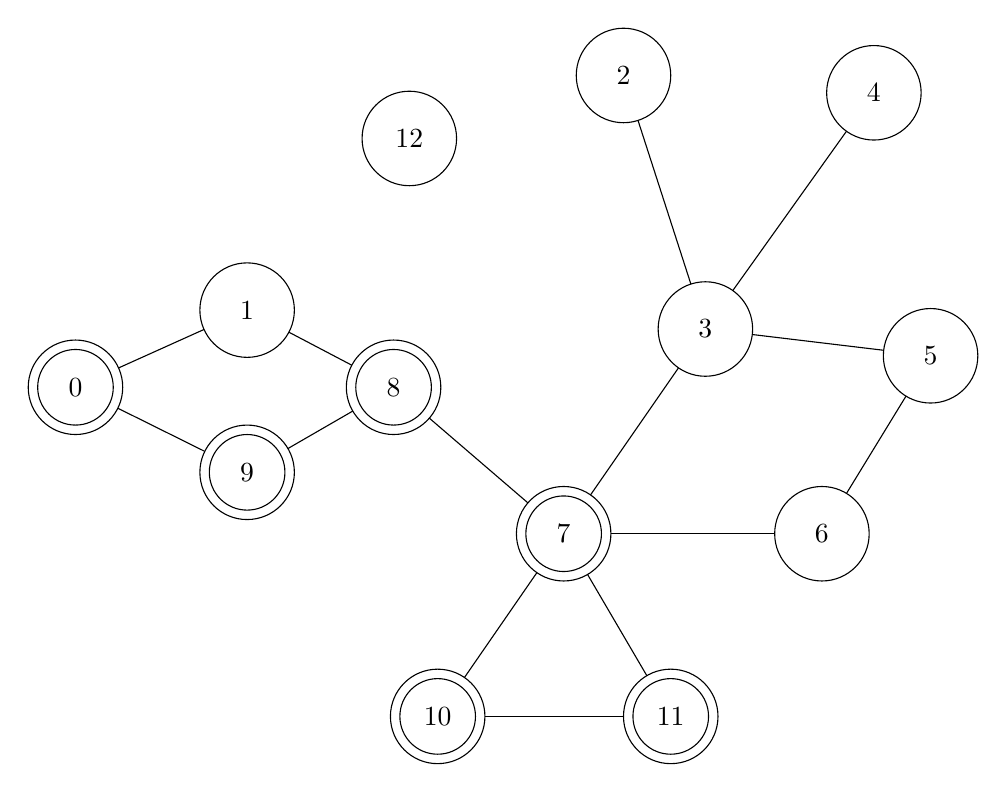
\begin{tikzpicture}[scale=0.2]
    \tikzstyle{every node}+=[inner sep=0pt]
    \draw [black] (5.4,-28.9) circle (3);
    \draw (5.4,-28.9) node {$0$};
    \draw [black] (5.4,-28.9) circle (2.4);
    \draw [black] (16.3,-24) circle (3);
    \draw (16.3,-24) node {$1$};
    \draw [black] (16.3,-34.3) circle (3);
    \draw (16.3,-34.3) node {$9$};
    \draw [black] (16.3,-34.3) circle (2.4);
    \draw [black] (25.6,-28.9) circle (3);
    \draw (25.6,-28.9) node {$8$};
    \draw [black] (25.6,-28.9) circle (2.4);
    \draw [black] (36.4,-38.2) circle (3);
    \draw (36.4,-38.2) node {$7$};
    \draw [black] (36.4,-38.2) circle (2.4);
    \draw [black] (28.4,-49.8) circle (3);
    \draw (28.4,-49.8) node {$10$};
    \draw [black] (28.4,-49.8) circle (2.4);
    \draw [black] (43.2,-49.8) circle (3);
    \draw (43.2,-49.8) node {$11$};
    \draw [black] (43.2,-49.8) circle (2.4);
    \draw [black] (52.8,-38.2) circle (3);
    \draw (52.8,-38.2) node {$6$};
    \draw [black] (59.7,-26.9) circle (3);
    \draw (59.7,-26.9) node {$5$};
    \draw [black] (45.4,-25.2) circle (3);
    \draw (45.4,-25.2) node {$3$};
    \draw [black] (56.1,-10.2) circle (3);
    \draw (56.1,-10.2) node {$4$};
    \draw [black] (40.2,-9.1) circle (3);
    \draw (40.2,-9.1) node {$2$};
    \draw [black] (26.6,-13.1) circle (3);
    \draw (26.6,-13.1) node {$12$};
    \draw [black] (8.14,-27.67) -- (13.56,-25.23);
    \draw [black] (8.09,-30.23) -- (13.61,-32.97);
    \draw [black] (18.95,-25.4) -- (22.95,-27.5);
    \draw [black] (18.89,-32.79) -- (23.01,-30.41);
    \draw [black] (27.87,-30.86) -- (34.13,-36.24);
    \draw [black] (34.7,-40.67) -- (30.1,-47.33);
    \draw [black] (37.92,-40.79) -- (41.68,-47.21);
    \draw [black] (31.4,-49.8) -- (40.2,-49.8);
    \draw [black] (39.4,-38.2) -- (49.8,-38.2);
    \draw [black] (38.11,-35.73) -- (43.69,-27.67);
    \draw [black] (48.38,-25.55) -- (56.72,-26.55);
    \draw [black] (54.36,-35.64) -- (58.14,-29.46);
    \draw [black] (47.14,-22.76) -- (54.36,-12.64);
    \draw [black] (44.48,-22.35) -- (41.12,-11.95);
    \end{tikzpicture}
\end{center}
\end{figure}

We already visited the node 7, so we need to return using backtracking an visit the rest of neighbours of node 7 so we continue doing the DFS but in another direction and we put a mark in the nodes that we already visited but are not valid.

\begin{figure}[H]
\begin{center}
    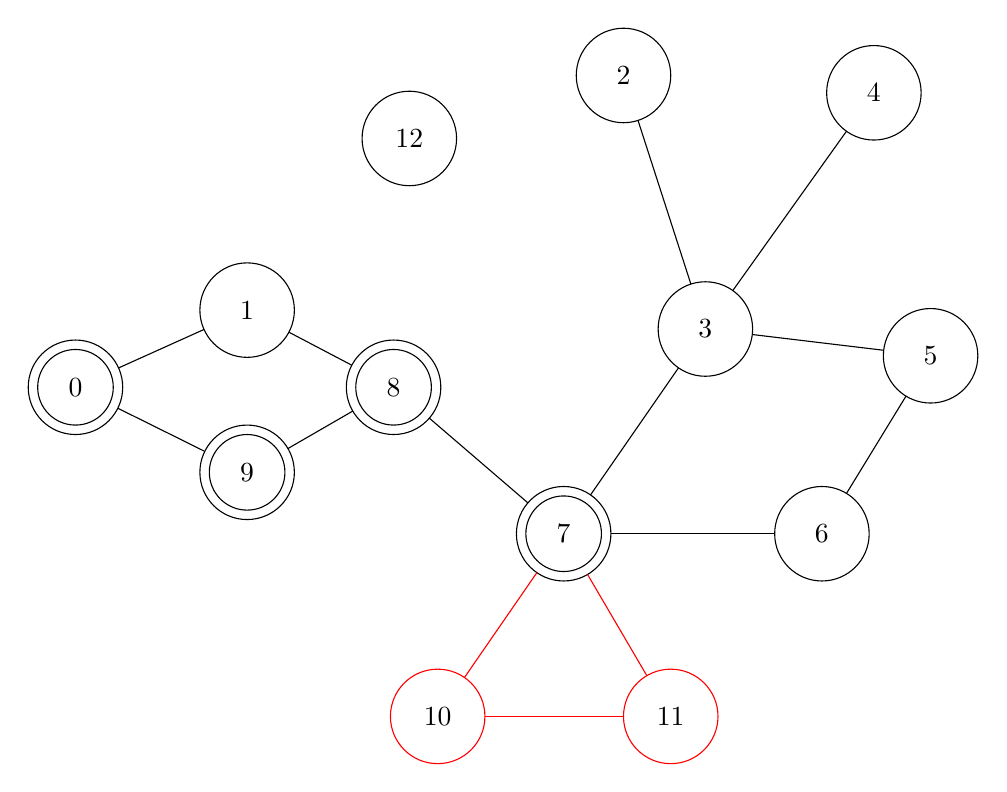
\begin{tikzpicture}[scale=0.2]
    \tikzstyle{every node}+=[inner sep=0pt]
    \draw [black] (5.4,-28.9) circle (3);
    \draw (5.4,-28.9) node {$0$};
    \draw [black] (5.4,-28.9) circle (2.4);
    \draw [black] (16.3,-24) circle (3);
    \draw (16.3,-24) node {$1$};
    \draw [black] (16.3,-34.3) circle (3);
    \draw (16.3,-34.3) node {$9$};
    \draw [black] (16.3,-34.3) circle (2.4);
    \draw [black] (25.6,-28.9) circle (3);
    \draw (25.6,-28.9) node {$8$};
    \draw [black] (25.6,-28.9) circle (2.4);
    \draw [black] (36.4,-38.2) circle (3);
    \draw (36.4,-38.2) node {$7$};
    \draw [black] (36.4,-38.2) circle (2.4);
    \draw [red] (28.4,-49.8) circle (3);
    \draw (28.4,-49.8) node {$10$};
    \draw [red] (43.2,-49.8) circle (3);
    \draw (43.2,-49.8) node {$11$};
    \draw [black] (52.8,-38.2) circle (3);
    \draw (52.8,-38.2) node {$6$};
    \draw [black] (59.7,-26.9) circle (3);
    \draw (59.7,-26.9) node {$5$};
    \draw [black] (45.4,-25.2) circle (3);
    \draw (45.4,-25.2) node {$3$};
    \draw [black] (56.1,-10.2) circle (3);
    \draw (56.1,-10.2) node {$4$};
    \draw [black] (40.2,-9.1) circle (3);
    \draw (40.2,-9.1) node {$2$};
    \draw [black] (26.6,-13.1) circle (3);
    \draw (26.6,-13.1) node {$12$};
    \draw [black] (8.14,-27.67) -- (13.56,-25.23);
    \draw [black] (8.09,-30.23) -- (13.61,-32.97);
    \draw [black] (18.95,-25.4) -- (22.95,-27.5);
    \draw [black] (18.89,-32.79) -- (23.01,-30.41);
    \draw [black] (27.87,-30.86) -- (34.13,-36.24);
    \draw [red] (34.7,-40.67) -- (30.1,-47.33);
    \draw [red] (37.92,-40.79) -- (41.68,-47.21);
    \draw [red] (31.4,-49.8) -- (40.2,-49.8);
    \draw [black] (39.4,-38.2) -- (49.8,-38.2);
    \draw [black] (38.11,-35.73) -- (43.69,-27.67);
    \draw [black] (48.38,-25.55) -- (56.72,-26.55);
    \draw [black] (54.36,-35.64) -- (58.14,-29.46);
    \draw [black] (47.14,-22.76) -- (54.36,-12.64);
    \draw [black] (44.48,-22.35) -- (41.12,-11.95);
    \end{tikzpicture}
\end{center}
\end{figure}

Now we move to the node 3 and then to the node 2 so we need to make backtracking again and continue with our DFS

\begin{figure}[H]
\begin{center}
    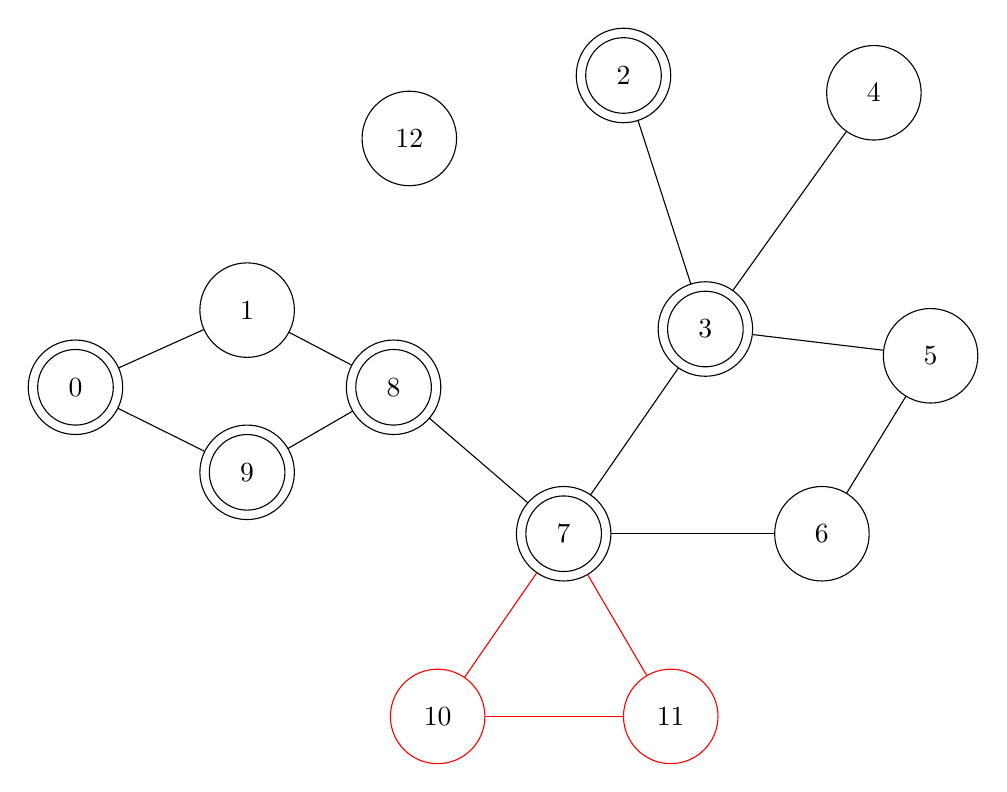
\begin{tikzpicture}[scale=0.2]
    \tikzstyle{every node}+=[inner sep=0pt]
    \draw [black] (5.4,-28.9) circle (3);
    \draw (5.4,-28.9) node {$0$};
    \draw [black] (5.4,-28.9) circle (2.4);
    \draw [black] (16.3,-24) circle (3);
    \draw (16.3,-24) node {$1$};
    \draw [black] (16.3,-34.3) circle (3);
    \draw (16.3,-34.3) node {$9$};
    \draw [black] (16.3,-34.3) circle (2.4);
    \draw [black] (25.6,-28.9) circle (3);
    \draw (25.6,-28.9) node {$8$};
    \draw [black] (25.6,-28.9) circle (2.4);
    \draw [black] (36.4,-38.2) circle (3);
    \draw (36.4,-38.2) node {$7$};
    \draw [black] (36.4,-38.2) circle (2.4);
    \draw [red] (28.4,-49.8) circle (3);
    \draw (28.4,-49.8) node {$10$};
    \draw [red] (43.2,-49.8) circle (3);
    \draw (43.2,-49.8) node {$11$};
    \draw [black] (52.8,-38.2) circle (3);
    \draw (52.8,-38.2) node {$6$};
    \draw [black] (59.7,-26.9) circle (3);
    \draw (59.7,-26.9) node {$5$};
    \draw [black] (45.4,-25.2) circle (3);
    \draw (45.4,-25.2) node {$3$};
    \draw [black] (45.4,-25.2) circle (2.4);
    \draw [black] (56.1,-10.2) circle (3);
    \draw (56.1,-10.2) node {$4$};
    \draw [black] (40.2,-9.1) circle (3);
    \draw (40.2,-9.1) node {$2$};
    \draw [black] (40.2,-9.1) circle (2.4);
    \draw [black] (26.6,-13.1) circle (3);
    \draw (26.6,-13.1) node {$12$};
    \draw [black] (8.14,-27.67) -- (13.56,-25.23);
    \draw [black] (8.09,-30.23) -- (13.61,-32.97);
    \draw [black] (18.95,-25.4) -- (22.95,-27.5);
    \draw [black] (18.89,-32.79) -- (23.01,-30.41);
    \draw [black] (27.87,-30.86) -- (34.13,-36.24);
    \draw [red] (34.7,-40.67) -- (30.1,-47.33);
    \draw [red] (37.92,-40.79) -- (41.68,-47.21);
    \draw [red] (31.4,-49.8) -- (40.2,-49.8);
    \draw [black] (39.4,-38.2) -- (49.8,-38.2);
    \draw [black] (38.11,-35.73) -- (43.69,-27.67);
    \draw [black] (48.38,-25.55) -- (56.72,-26.55);
    \draw [black] (54.36,-35.64) -- (58.14,-29.46);
    \draw [black] (47.14,-22.76) -- (54.36,-12.64);
    \draw [black] (44.48,-22.35) -- (41.12,-11.95);
    \end{tikzpicture}
\end{center}
\end{figure}

Now we move to the node 4 but again it is a dead end so we move to the node 5 then to the node 6, then to the node 7 but we already visited

\begin{figure}[H]
\begin{center}
    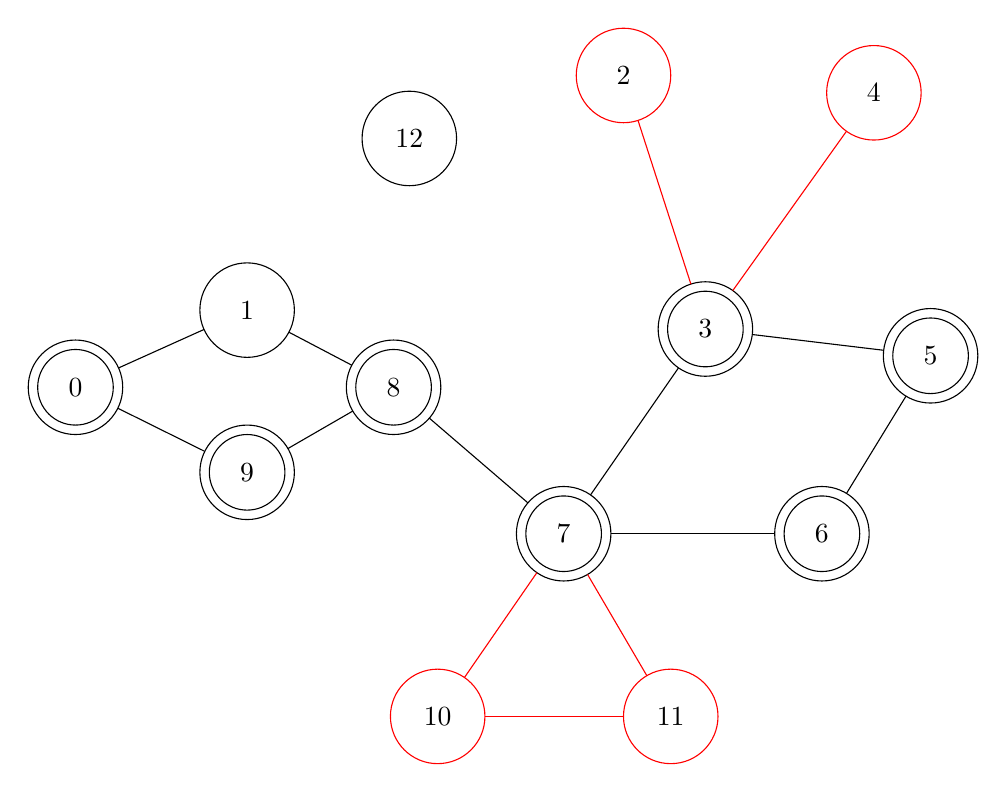
\begin{tikzpicture}[scale=0.2]
    \tikzstyle{every node}+=[inner sep=0pt]
    \draw [black] (5.4,-28.9) circle (3);
    \draw (5.4,-28.9) node {$0$};
    \draw [black] (5.4,-28.9) circle (2.4);
    \draw [black] (16.3,-24) circle (3);
    \draw (16.3,-24) node {$1$};
    \draw [black] (16.3,-34.3) circle (3);
    \draw (16.3,-34.3) node {$9$};
    \draw [black] (16.3,-34.3) circle (2.4);
    \draw [black] (25.6,-28.9) circle (3);
    \draw (25.6,-28.9) node {$8$};
    \draw [black] (25.6,-28.9) circle (2.4);
    \draw [black] (36.4,-38.2) circle (3);
    \draw (36.4,-38.2) node {$7$};
    \draw [black] (36.4,-38.2) circle (2.4);
    \draw [red] (28.4,-49.8) circle (3);
    \draw (28.4,-49.8) node {$10$};
    \draw [red] (43.2,-49.8) circle (3);
    \draw (43.2,-49.8) node {$11$};
    \draw [black] (52.8,-38.2) circle (3);
    \draw (52.8,-38.2) node {$6$};
    \draw [black] (52.8,-38.2) circle (2.4);
    \draw [black] (59.7,-26.9) circle (3);
    \draw (59.7,-26.9) node {$5$};
    \draw [black] (59.7,-26.9) circle (2.4);
    \draw [black] (45.4,-25.2) circle (3);
    \draw (45.4,-25.2) node {$3$};
    \draw [black] (45.4,-25.2) circle (2.4);
    \draw [red] (56.1,-10.2) circle (3);
    \draw (56.1,-10.2) node {$4$};
    \draw [red] (40.2,-9.1) circle (3);
    \draw (40.2,-9.1) node {$2$};
    \draw [black] (26.6,-13.1) circle (3);
    \draw (26.6,-13.1) node {$12$};
    \draw [black] (8.14,-27.67) -- (13.56,-25.23);
    \draw [black] (8.09,-30.23) -- (13.61,-32.97);
    \draw [black] (18.95,-25.4) -- (22.95,-27.5);
    \draw [black] (18.89,-32.79) -- (23.01,-30.41);
    \draw [black] (27.87,-30.86) -- (34.13,-36.24);
    \draw [red] (34.7,-40.67) -- (30.1,-47.33);
    \draw [red] (37.92,-40.79) -- (41.68,-47.21);
    \draw [red] (31.4,-49.8) -- (40.2,-49.8);
    \draw [black] (39.4,-38.2) -- (49.8,-38.2);
    \draw [black] (38.11,-35.73) -- (43.69,-27.67);
    \draw [black] (48.38,-25.55) -- (56.72,-26.55);
    \draw [black] (54.36,-35.64) -- (58.14,-29.46);
    \draw [red] (47.14,-22.76) -- (54.36,-12.64);
    \draw [red] (44.48,-22.35) -- (41.12,-11.95);
    \end{tikzpicture}
\end{center}
\end{figure}

Now we backtrack and we return to the node 8, and we continue doing the DFS 

\begin{figure}[H]
\begin{center}
    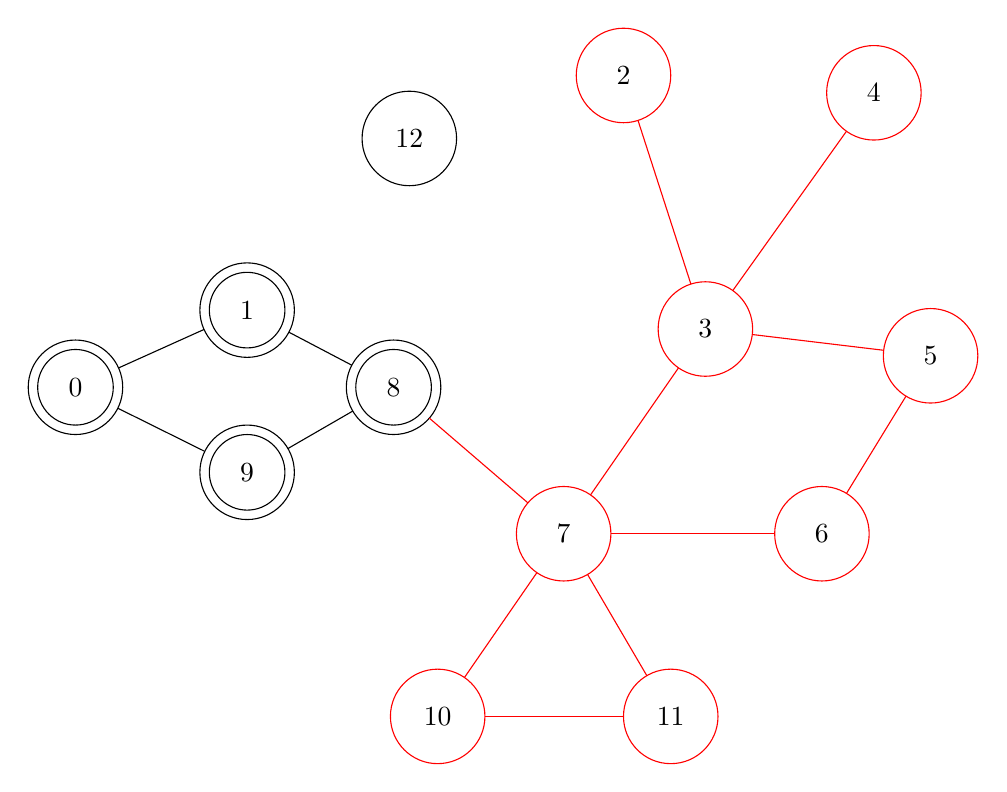
\begin{tikzpicture}[scale=0.2]
    \tikzstyle{every node}+=[inner sep=0pt]
    \draw [black] (5.4,-28.9) circle (3);
    \draw (5.4,-28.9) node {$0$};
    \draw [black] (5.4,-28.9) circle (2.4);
    \draw [black] (16.3,-24) circle (3);
    \draw (16.3,-24) node {$1$};
    \draw [black] (16.3,-24) circle (2.4);
    \draw [black] (16.3,-34.3) circle (3);
    \draw (16.3,-34.3) node {$9$};
    \draw [black] (16.3,-34.3) circle (2.4);
    \draw [black] (25.6,-28.9) circle (3);
    \draw (25.6,-28.9) node {$8$};
    \draw [black] (25.6,-28.9) circle (2.4);
    \draw [red] (36.4,-38.2) circle (3);
    \draw (36.4,-38.2) node {$7$};
    \draw [red] (28.4,-49.8) circle (3);
    \draw (28.4,-49.8) node {$10$};
    \draw [red] (43.2,-49.8) circle (3);
    \draw (43.2,-49.8) node {$11$};
    \draw [red] (52.8,-38.2) circle (3);
    \draw (52.8,-38.2) node {$6$};
    \draw [red] (59.7,-26.9) circle (3);
    \draw (59.7,-26.9) node {$5$};
    \draw [red] (45.4,-25.2) circle (3);
    \draw (45.4,-25.2) node {$3$};
    \draw [red] (56.1,-10.2) circle (3);
    \draw (56.1,-10.2) node {$4$};
    \draw [red] (40.2,-9.1) circle (3);
    \draw (40.2,-9.1) node {$2$};
    \draw [black] (26.6,-13.1) circle (3);
    \draw (26.6,-13.1) node {$12$};
    \draw [black] (8.14,-27.67) -- (13.56,-25.23);
    \draw [black] (8.09,-30.23) -- (13.61,-32.97);
    \draw [black] (18.95,-25.4) -- (22.95,-27.5);
    \draw [black] (18.89,-32.79) -- (23.01,-30.41);
    \draw [red] (27.87,-30.86) -- (34.13,-36.24);
    \draw [red] (34.7,-40.67) -- (30.1,-47.33);
    \draw [red] (37.92,-40.79) -- (41.68,-47.21);
    \draw [red] (31.4,-49.8) -- (40.2,-49.8);
    \draw [red] (39.4,-38.2) -- (49.8,-38.2);
    \draw [red] (38.11,-35.73) -- (43.69,-27.67);
    \draw [red] (48.38,-25.55) -- (56.72,-26.55);
    \draw [red] (54.36,-35.64) -- (58.14,-29.46);
    \draw [red] (47.14,-22.76) -- (54.36,-12.64);
    \draw [red] (44.48,-22.35) -- (41.12,-11.95);
    \end{tikzpicture}
\end{center}
\end{figure}